\documentclass[12pt]{article}
\usepackage{polski}
\usepackage[utf8]{inputenc}
\usepackage[T1]{fontenc}
\usepackage{times}

\usepackage{amsfonts}
\usepackage{amsmath}
\usepackage{bm}
\usepackage{mathtools}
\mathtoolsset{showonlyrefs}


\usepackage{tabularx}
\usepackage{array}
\newcolumntype{Y}{>{\centering\arraybackslash}X}
\newcolumntype{Z}{>{\centering\arraybackslash}p}
\usepackage{multirow}
\usepackage{hyperref}

\usepackage{enumitem}
\usepackage{float}


\usepackage{graphicx}
\usepackage{rotating}
\usepackage{subcaption}


%\usepackage{animate}

\renewcommand{\thesection}{\arabic{section}}
\renewcommand{\thesubsection}{\arabic{section}.\arabic{subsection}}
\usepackage{wrapfig}



\usepackage{amsmath}
\usepackage{amsthm}
\usepackage{dsfont}
\newtheorem{lema}{Lemma}

\newtheoremstyle{exer}{20pt}{10pt}{}{0pt}{\bfseries}{.\\}{.5em}{}
\theoremstyle{exer}
\newtheorem{ex}{Ex}

%\usepackage[a4paper,total={6in,10in}]{geometry}
\usepackage[a4paper,total={7in,10in}]{geometry}
%\newtheoremstyle{style name}{space above}{space below}{body font}{indent amount}{head font}{head punct}{after head space}{head spec}
\usepackage{color}

\begin{document}
	\begin{titlepage}
		\begin{center}
			
			\textbf{\Huge  Analiza danych rzeczywistych przy pomocy modelu ARMA}
			
			\vspace{0.5cm}
			
			\vspace{1.5cm}
			
			\textbf{\LARGE Autorzy}\\
			\vspace{0.5cm}
			\large Kacper Budnik, 262286\\
			\large Maciej Karczewski, 262282\\
			
			
			\vfill
			
			\vspace{0.4cm}
				
\includegraphics[width=0.60\textwidth]{img/logo.PNG}

			
			\vspace{0.8cm}
			Wydział Matematyki	
			\today
		\end{center}
	\end{titlepage}
	\tableofcontents
	\newpage
	
	\section{Wprowadzenie}
	Analizowane dane pochodzą ze strony \href{https://www.kaggle.com/code/amar09/time-series-delhi-weather-forecasting-arima/data}{Kaggel}. Zawierają one dane pogodowe z Indyjskiego miasta Delhi od dnia 1 listopada 1996 do 24 kwiecień 2017. Dane były pobierane w przynajmniej ośmiu ustalonych momentach dnia w odstępach trzygodzinnych. W pierwszych latach dane w większości były pobierane w odstępach godzinnych. Zawierają one informacje między innymi o wilogtności, temperaturze punktu rosy, zjawiskach atmosferycznych, czyli informacjie czy wystąpiły opady, burze, mgły i tym podobne oraz dacie pomiaru. Przykładowe dane przezentują się następująco.
	\begin{table}[H]
		\centering
		\begin{tabularx}{4\textwidth/5}{|p{3cm}|Y|Y|Y|Y|Y|}
			\hline
			datetime\_utc & \_dewptm & \_fog & \_hail & \_hum & \_tempm \\\hline
			19961101-11:00 &  9 & 0 & 0 & 27& 30 \\\hline
			19961101-12:00 &  10 & 0 & 0 & 32& 28 \\\hline
			19961101-13:00 &  11 & 0 & 0 & 44& 24 \\\hline
			19961101-14:00 &  10 & 0 & 0 & 41& 24 \\\hline
			19961101-16:00 &  11 & 0 & 0 & 47& 23 \\\hline
			19961101-17:00 &  12 & 0 & 0 & 56& 21 \\\hline
		\end{tabularx}
	\end{table}
	W analizie interesują nas jedynie kolumny \verb*|datetime_utc| przechowująca informację o dacie pomiaru oraz \verb*|_tempm| zawierająca odnotowaną temperaturę. Będziemy analizować zachowanie średniej temperatury dziennej w zależności od średnich z poprzednich dni.
	\section{Przygotowanie danych do analizy}
	Analizowane dane obejmują okres od listopada 1996 roku, jednak w pierwszych latach dane były pobierane w nieregularnie. Dlatego rozpatrujemy dane z okresu od 1 stycznia 2008 do 31 grudnia 2015 roku, równo 8 lat. Pozostałe dane tj. pochodzące z okresu 1 styczeń 2016 -- 24 kwiecień 2017 pozostawiliśmy jako dane testowe. W tych okresach pomiary były robione 8 razy dziennie, co 3 godziny każdy, rzadkie przypadki pomiarów w dodatkowych porach zostały pominięte. Za obserwacje odstające uznaliśmy te, które spełniają poniższą własność
	\begin{equation}
		y\notin\left(Q_1-1.5IQR,Q_3+1.5IQR\right),
	\end{equation}
	gdzie $y$ jest kandydatem na obserwacje odstającą, $Q_1$ i $Q_3$ to odpowiednio pierwszy i trzeci kwantyl, a $IQR$ jest rozstępem międzykwantylowym. W wyniku tej obserwacji odrzuciliśmy jedynie 4 obserwacje rzędu 90$^\circ$C. Pozostałe wyniki należą do przedziału od 1$^\circ$C do 47$^\circ$C. Naszym celem jest analiza średniej dziennej temperatury, zatem w kolejnym kroku obliczyliśmy tą średnią. Jej wartości mieszą się w przedziale od 6$^\circ$C do 40$^\circ$C. Uzyskane średnie temperatury rzeczywiście były osiągane w Indiach w odpowiednich czasach.
	\subsection{Sprawdzenie stacjonarności}	
	W celu sprawdzenia, czy nasze dane w postaci surowej są stacjonarne, posłużymy się testem ADF (Augmented Dickey-Fuller Test). W tym celu skorzystaliśmy z funkcji \verb*|ADFTest| z pakietu \verb*|HypothesisTests| dla języka \verb*|Julia|. Ponieważ nasze dane są pobierane codziennie, rozpatrywaliśmy lag do wartości 365. W ten sposób p-value=$0.2619$, zatem nie mamy podstaw do odrzucenia hipotezy zerowej głoszącej, że szereg nie jest stacjonarny.
	
	
	
	\section{Dekompozycja szeregu czasowego}
	\subsection{Wykresy dla surowych danych}
	Dekompozycję zaczniemy od analizy wykresów funkcji autokowariancji oraz częściowej autokowariancji. Prezentują się one następująco
	\begin{figure}[H]
		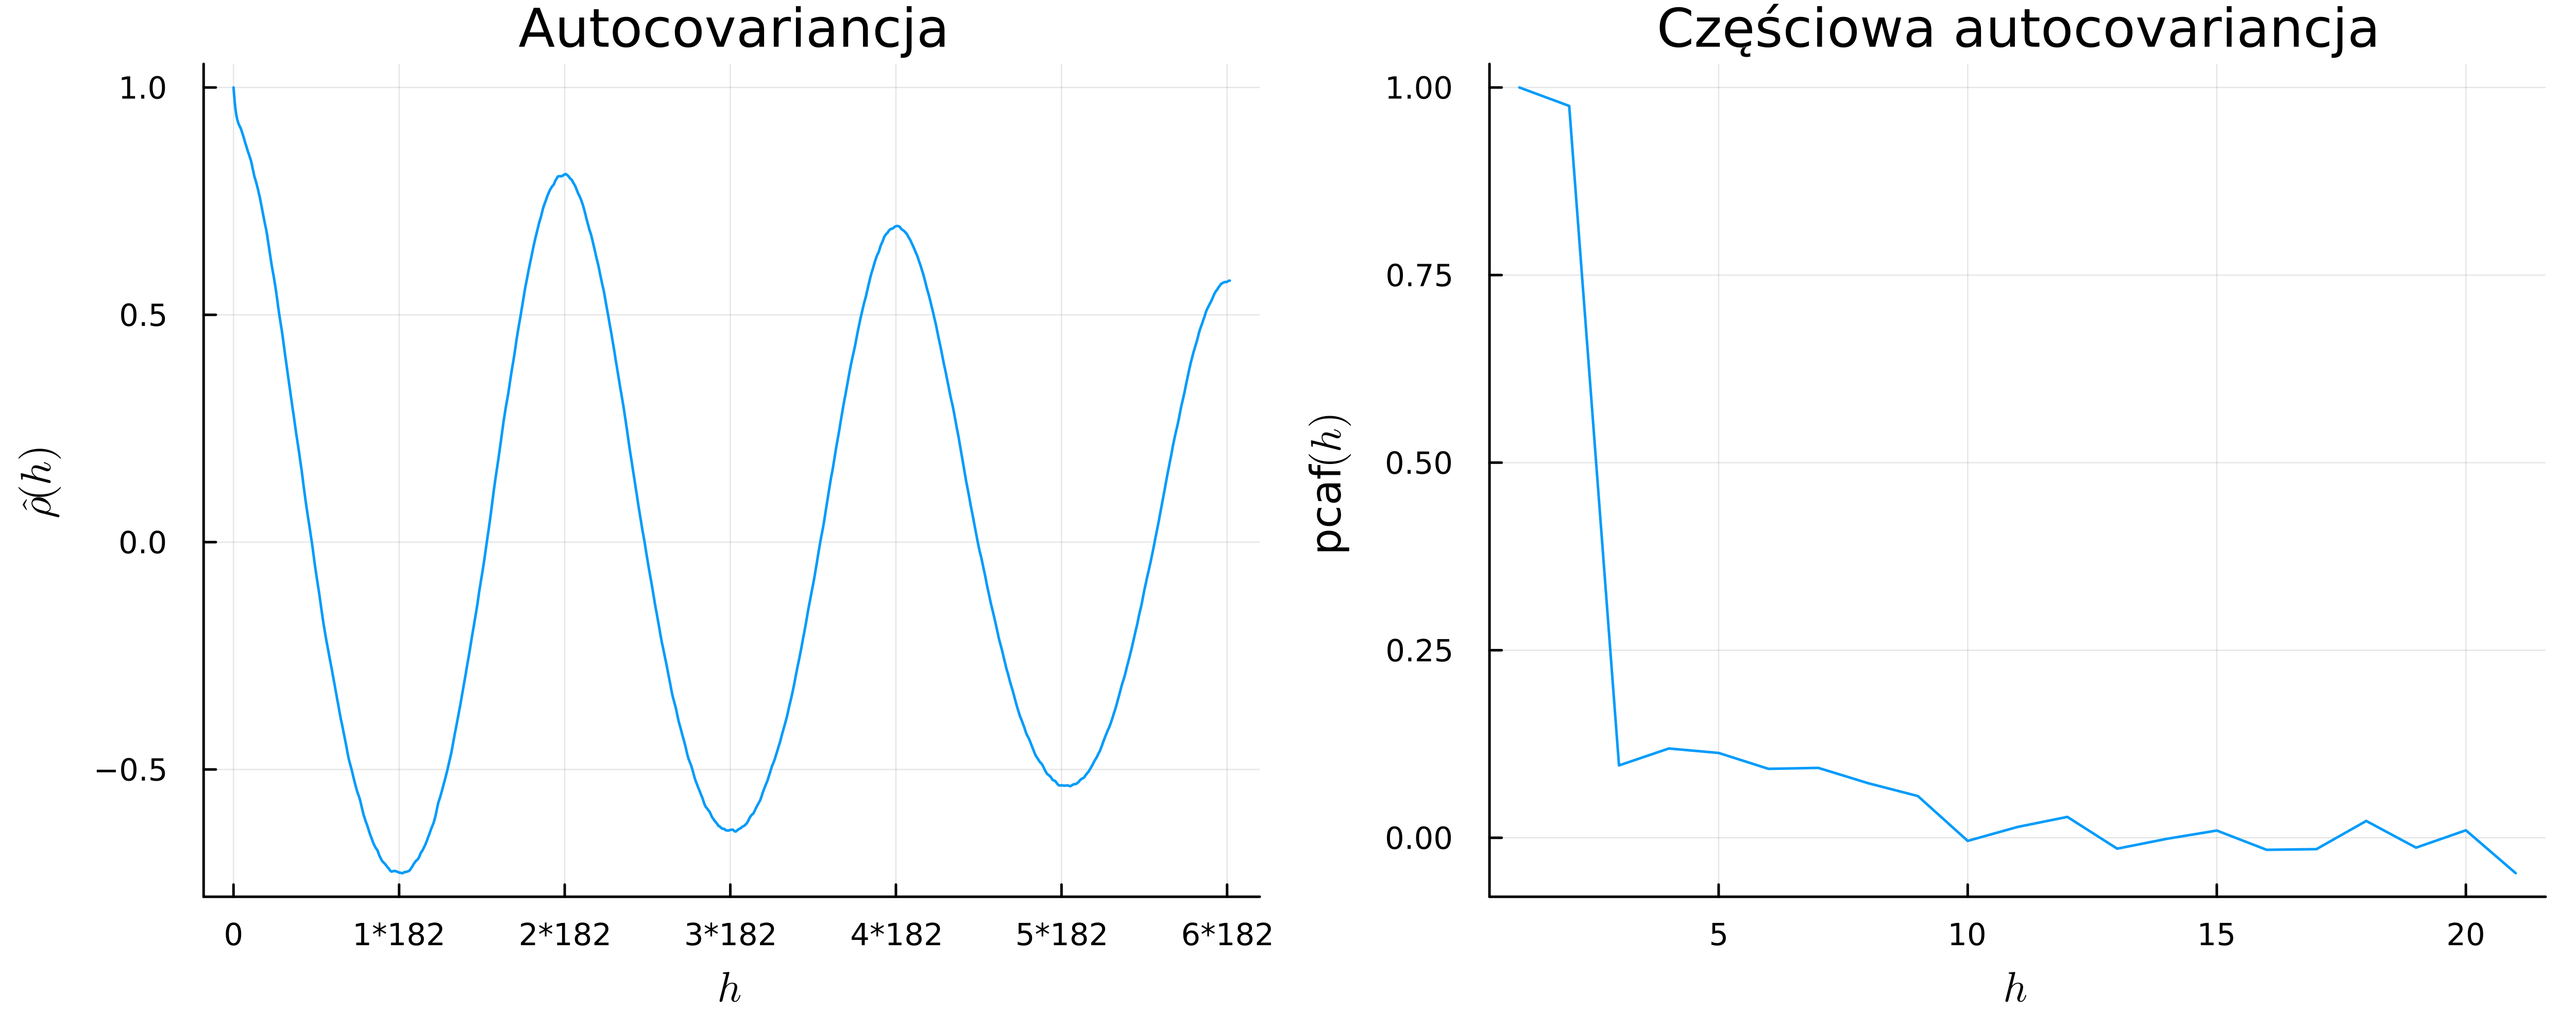
\includegraphics[width=\columnwidth]{Budnik/img/auto_dry.png}
		\caption{Funkcjie empircznej autokowariancji i częściowej autokowariancji.}\label{fig:dry_cov}
	\end{figure}
	Na powyższym wykresie widać okresowe zachowanie funkcji autokowariancji z okresem około 365. Liczba ta pokrywa się z liczbą dni w roku, co wydaje się intuicyjne. Z powodu na globalne ocieplenie możemy podejrzewać, że będzie istniał dodatni trend. Rzeczywiście, korzystając z funkcji \verb*|polyfit|, otrzymaliśmy trend
	\begin{equation}
		m(h)=24.8564+9\cdot10^{-5}h,
	\end{equation}  
	gdzie $m$ oznacza zmianę średniej temperatury w ciągu dnia. Zatem w ciągu 10 lat średnia temperatura w Delhi, według naszych obliczeń, wzrosła w przybliżeniu o $m(10\cdot365)-m(0)\approx0.3287^\circ$C. Według danych w tym samym okresie średnia temperatura na ziemi wzrosła, w zależności od regionu i źródeł, o więcej niż $0.2^\circ$C, zatem nasze wyniki częściowo pokrywają się z obserwowanymi zdarzeniami.
%	\subsection{Transformacja Boxa-Coxa}
%	Przed przystąpieniem do dekompozycji zastosowaliśmy transformację Boxa-Coxa. Transformacja ma ta na celu zminimalizowanie wariancji i przybliżenie rozkładu do rozkładku normalnego. Przy pomocy metod numerycznych oszacowaliśmy, że najmniejsza wariancja będzie dla transformacji z parametrem $\lambda\approx1.4591$, zatem analizować dane w postaci $y_n=x_n^\lambda$. Na poniższym histogramie widnieją dane przed transformacją (niebieski) oraz po transformacji (pomarańczowy).
%	\begin{figure}[H]
%		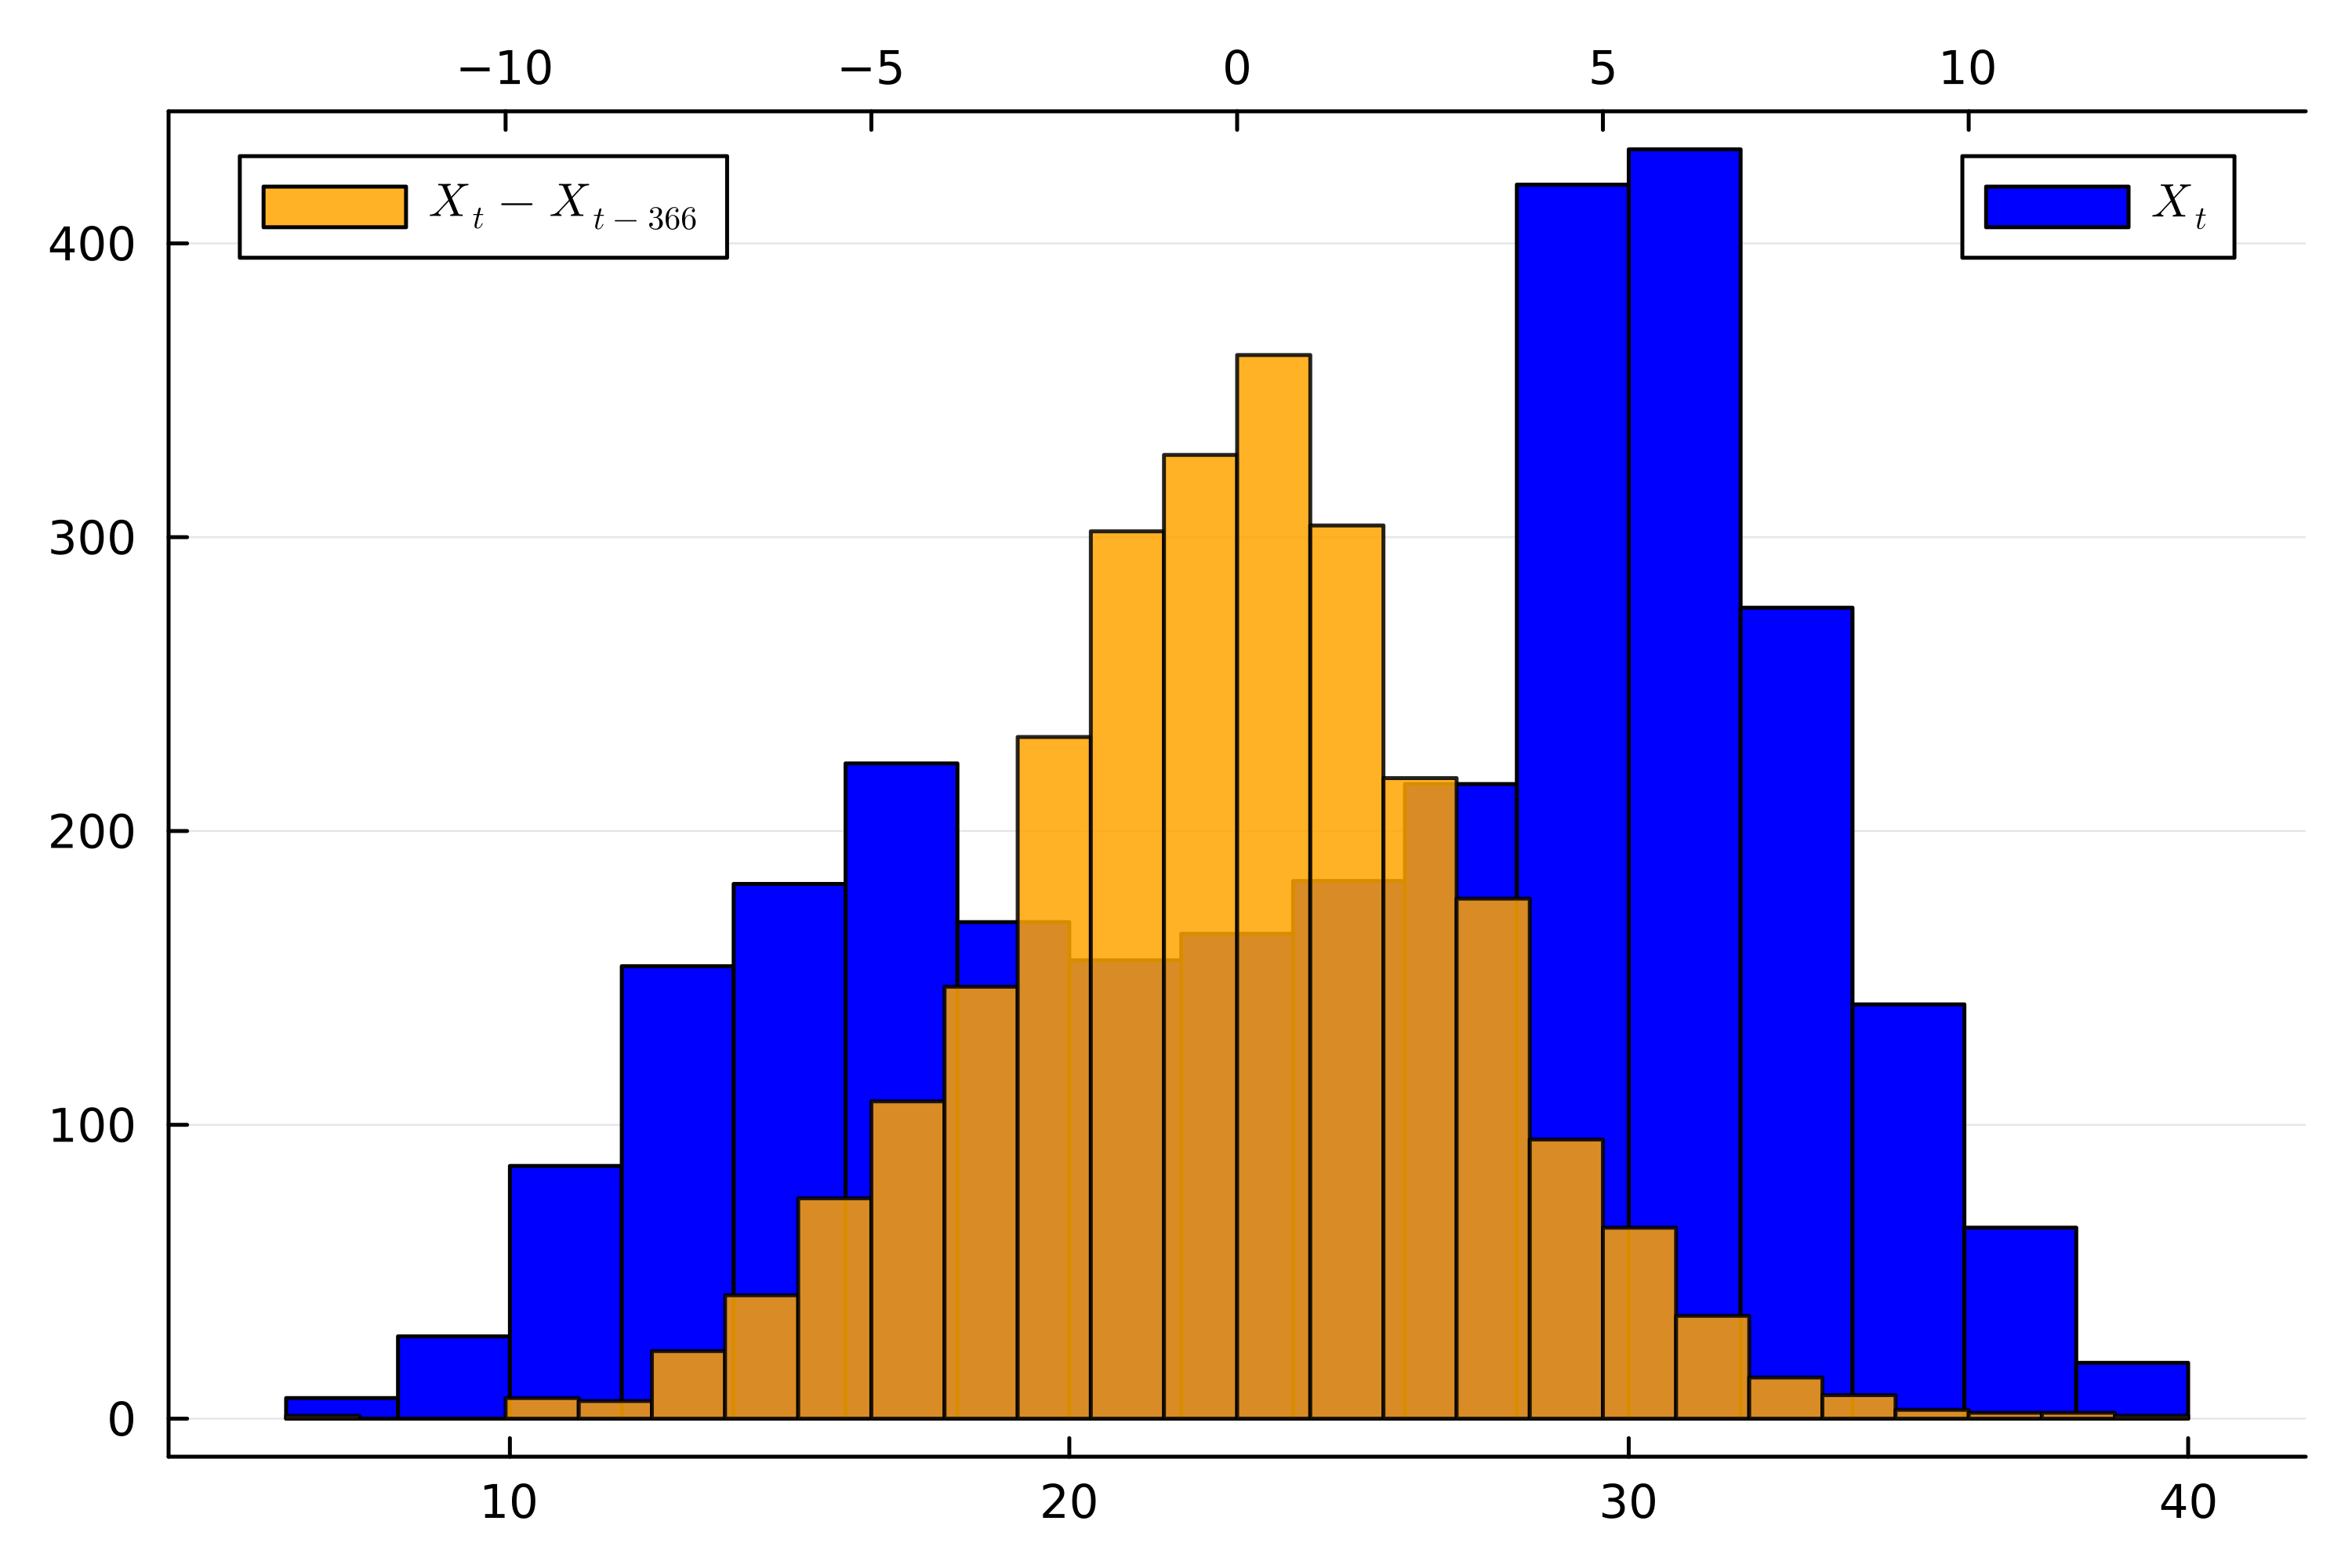
\includegraphics[width=\columnwidth]{Budnik/img/BoxCox.png}
%		\caption{Dane przed i po transformacji. Dolna oś wskazuje na dane oryginalne, na górze widnieje oś dla danych po transformacji.}
%	\end{figure}
	\subsection{Różnicowanie sezonowe}
	Tak jak już wspomnieliśmy, przy analizie wykresu \ref{fig:dry_cov}, nasze dane wykazują okresowość z okresem ok. 365 dni. By pozbyć się tych sezonowości zastosowaliśm różnicowanie sezonowe, czyli analizowaliśmy dalej dane w postaci
	\begin{equation}
		W_t=Y_t-Y_{t-a}.
	\end{equation}
	W naszym przypadku $a$ powinno być blisko $365$. Dokładną wartość $a=366$ dobraliśmy w taki sposób, by funkcjia autokowariancji była jak najmniejsza dla początkowych 10 wartości. Dla szeregu $W_t=Y_t-Y_{t-366}$ wygenerowaliśmy ponownie wykresy autokowariancji i częściowej autokowariacji.
	\begin{figure}[H]\label{fig:wet_cov}
		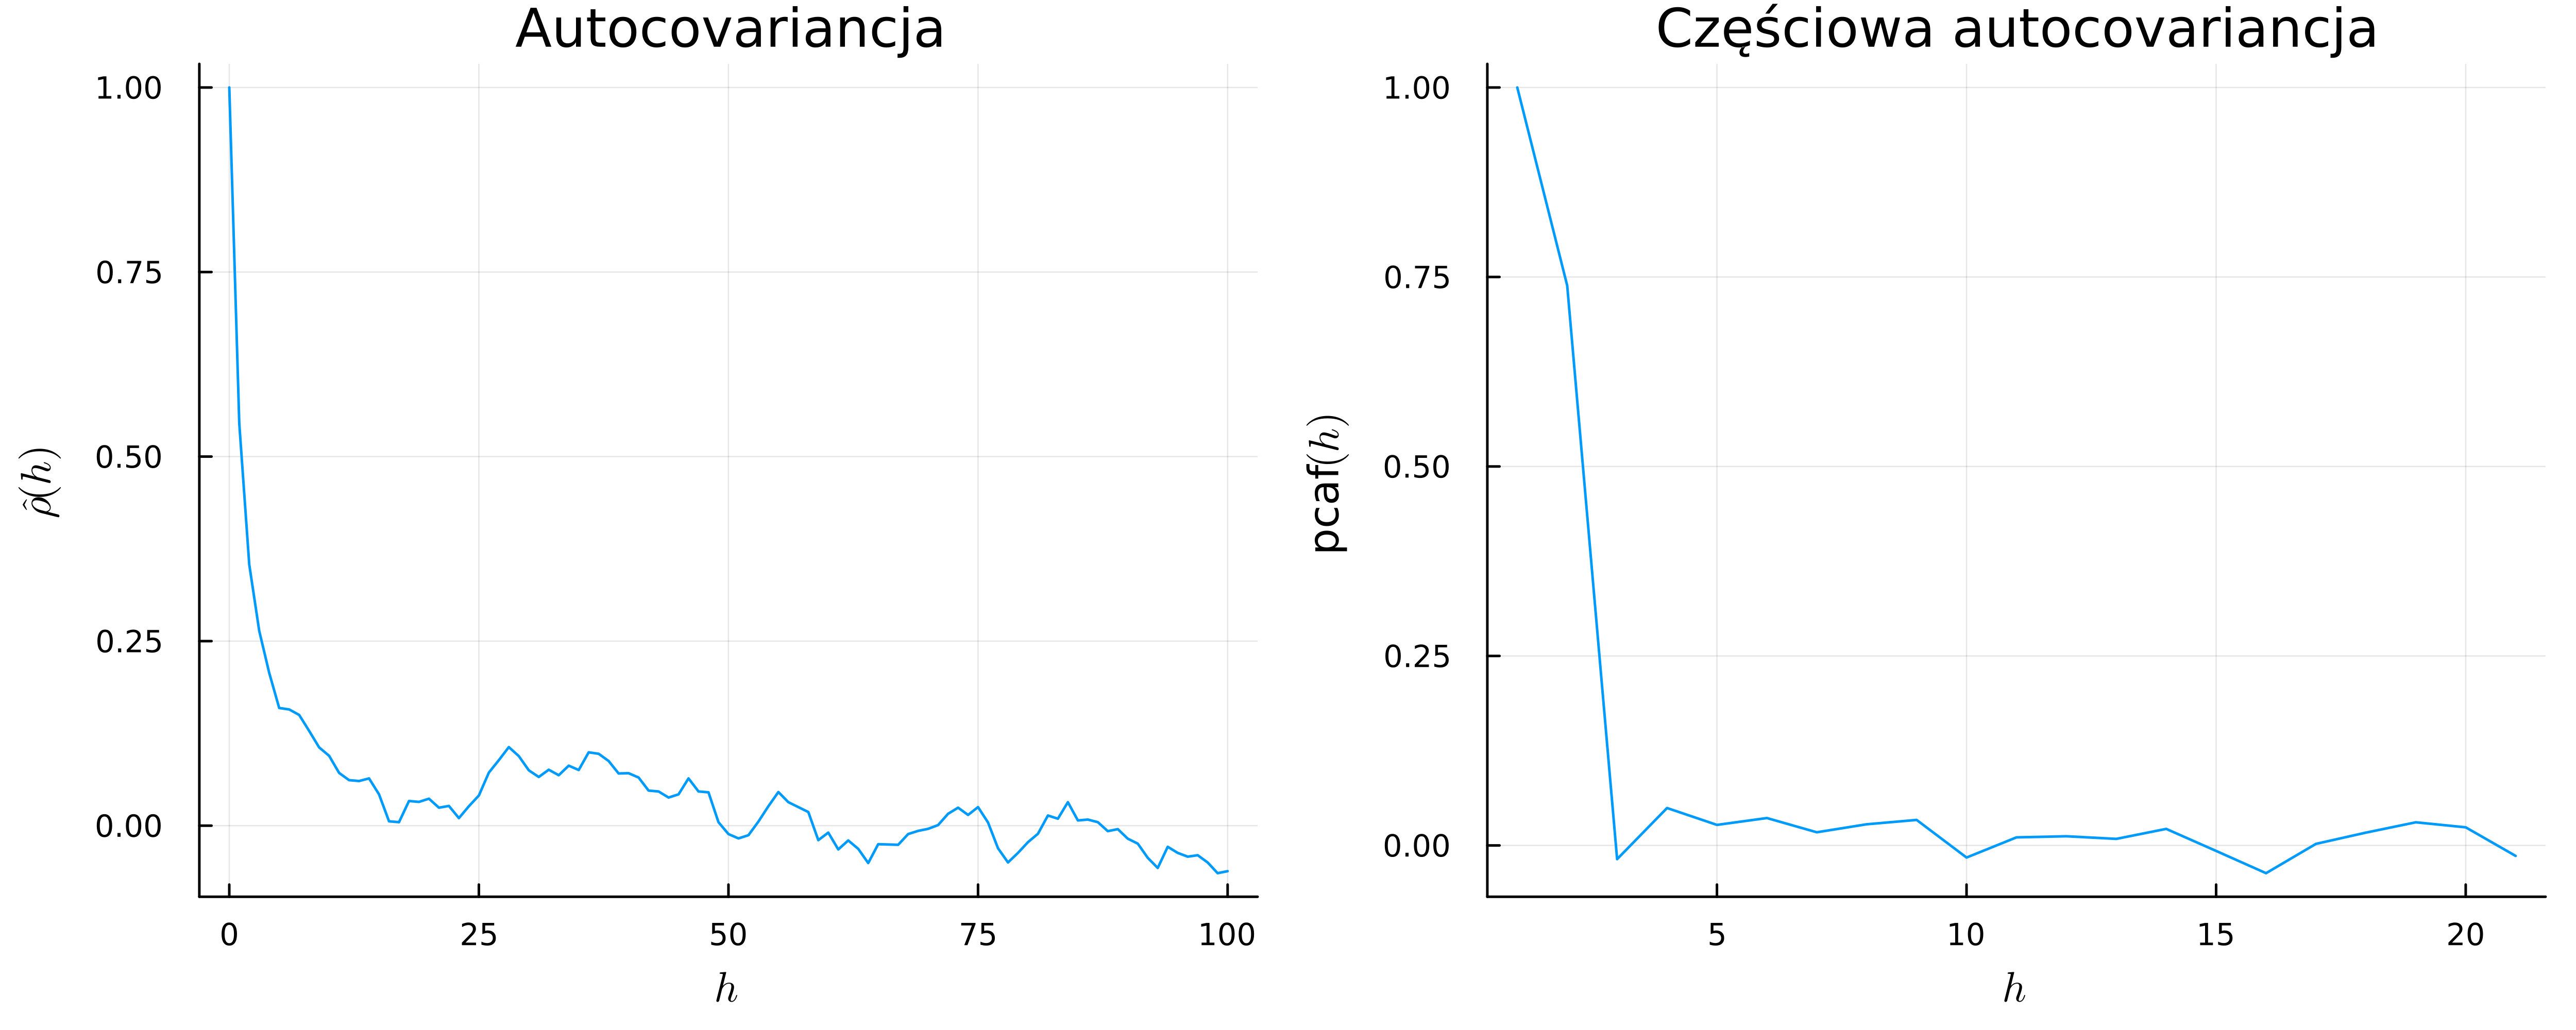
\includegraphics[width=\columnwidth]{Budnik/img/auto_wet.png}
		\caption{Funkcjie empircznej autokowariancji i częściowej autokowariancji.}
	\end{figure}
	Na wykresach widać, że funkcja częściowej i zwykłej autokowariancji szybko zbiega do wartości bliskich zeru i pozostaje w jego otoczeniu. Zatem możemy założyć, że nasz szereg jest już stacjonarny. By sprawdzić to założenie ponownie wykonaliśmy ADF-Test. W tym przypadku p-value$=0.002$, zatem możemy odrzucić hipotezę głoszącą, że szereg nie jest stacjonarny. Histogram naszych danych po transformacji wygląda następująco.
		\begin{figure}[H]
			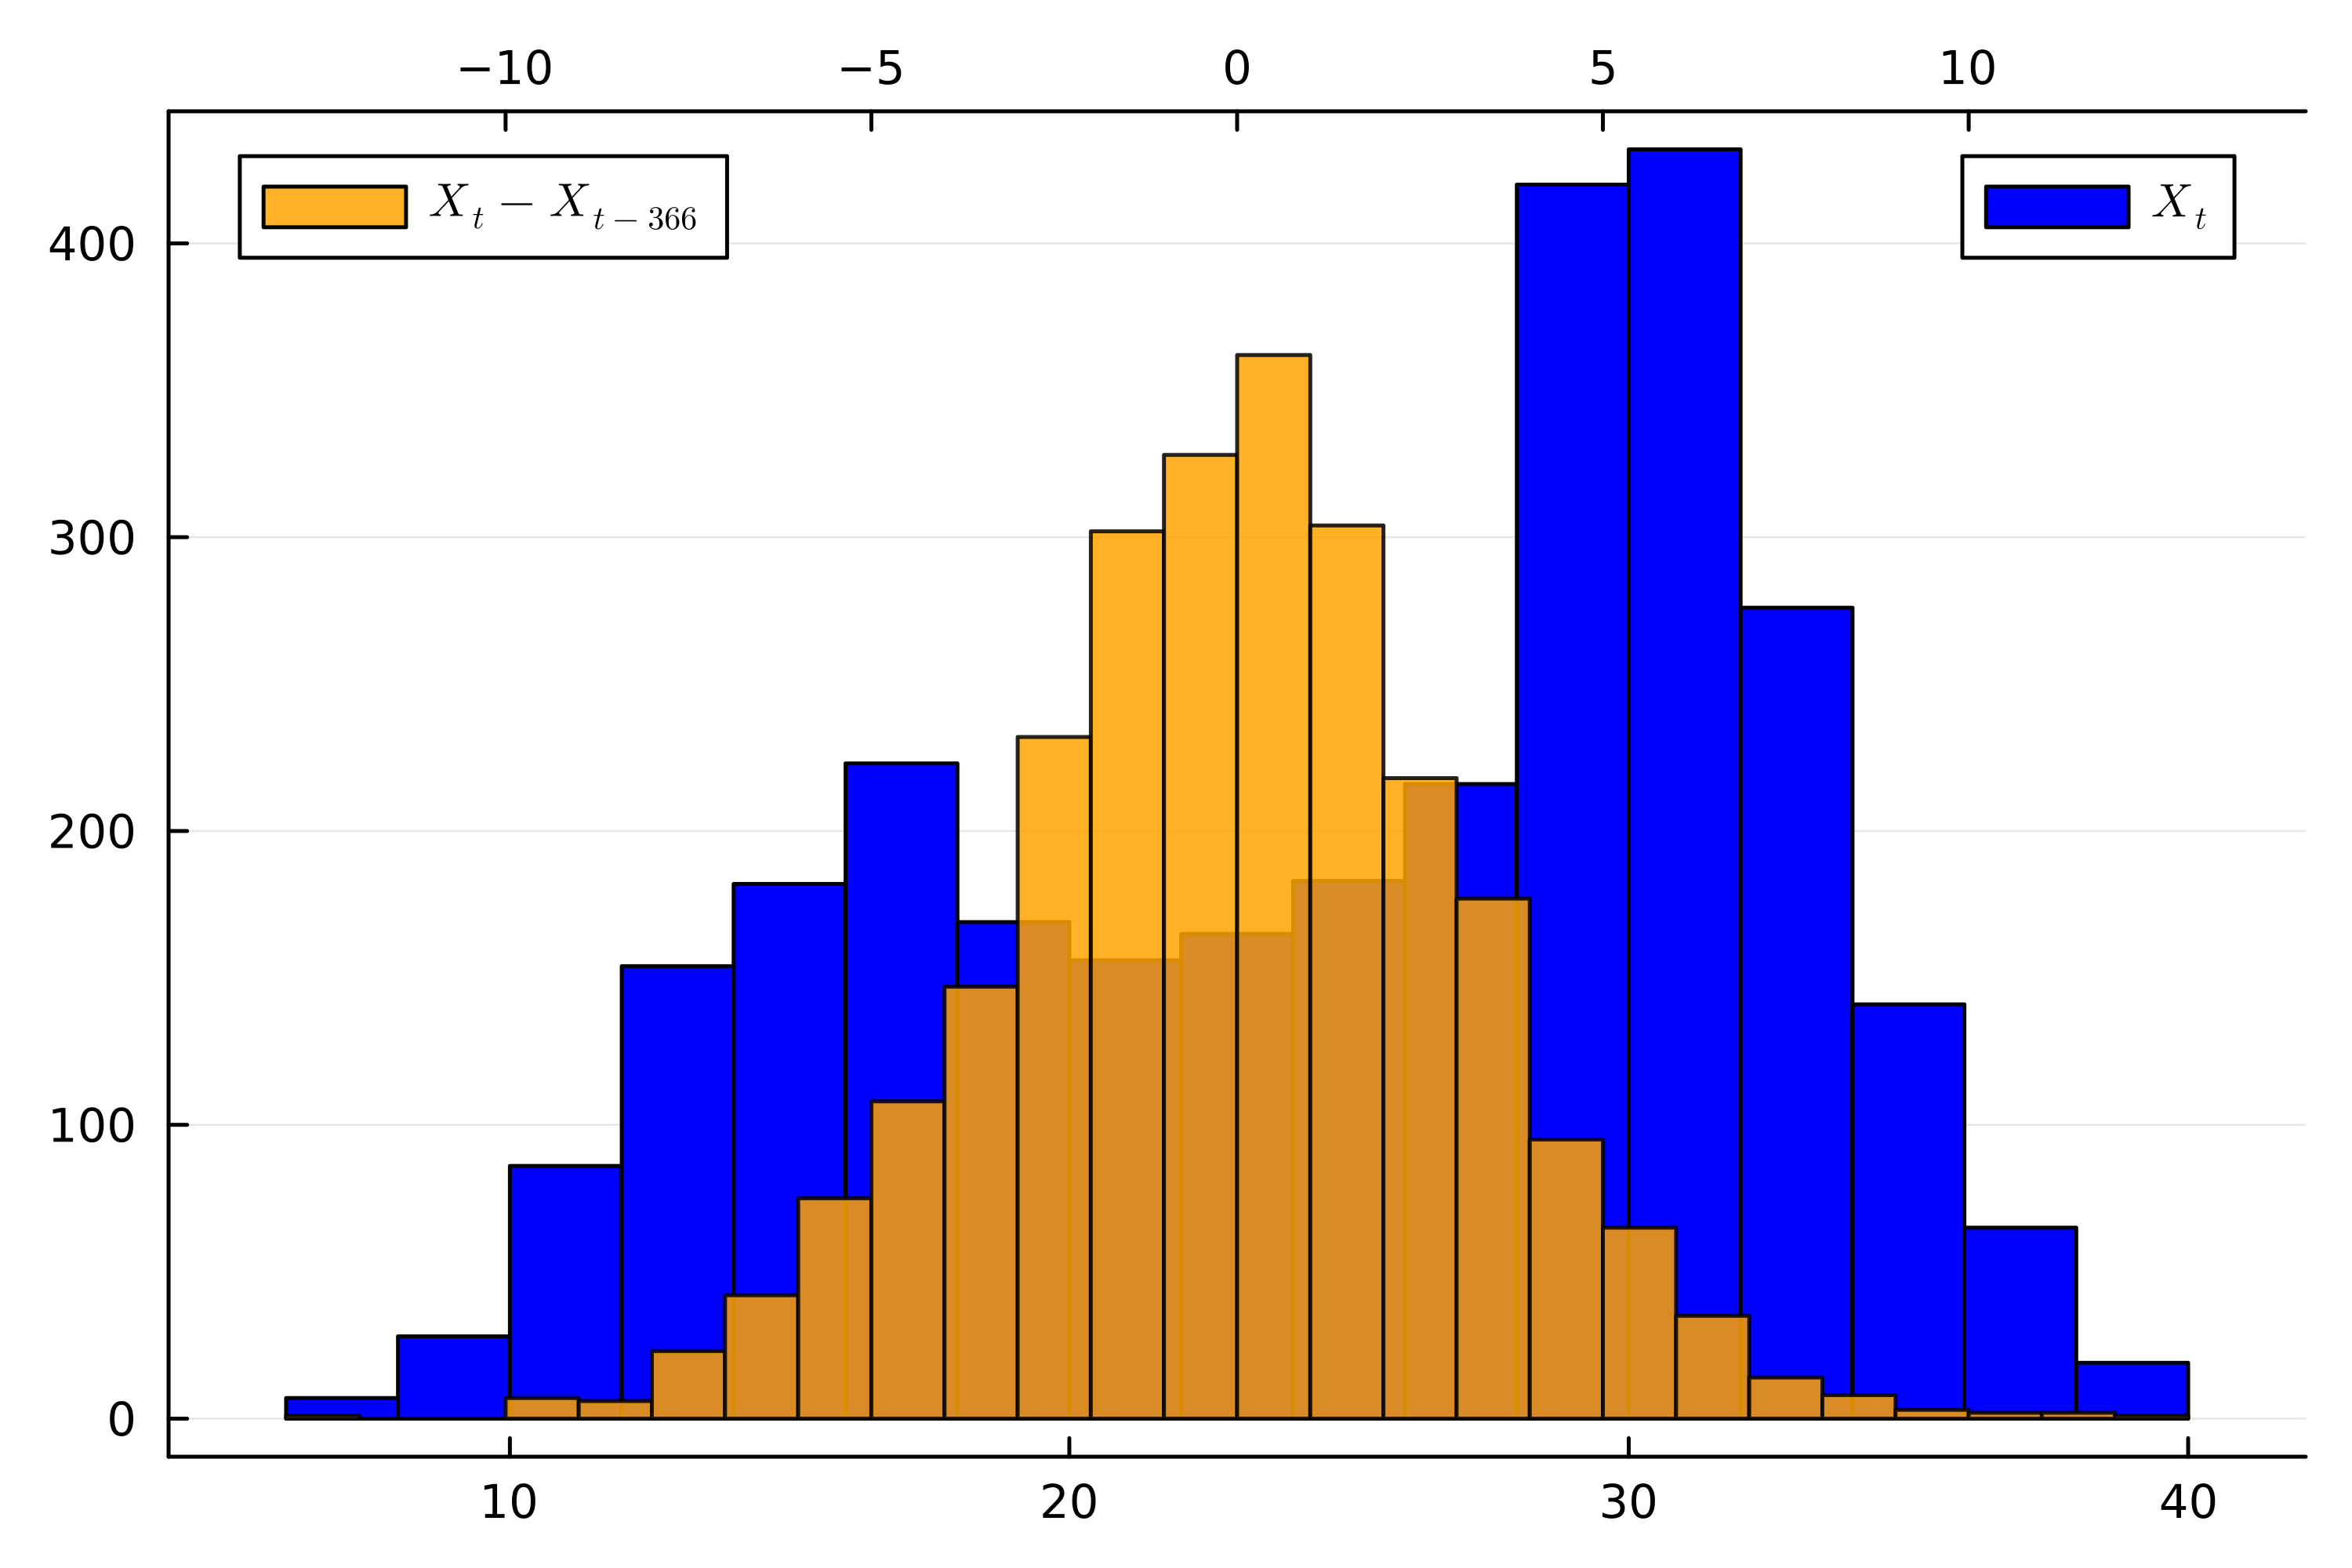
\includegraphics[width=\columnwidth]{Budnik/img/wet.png}
			\caption{Dane przed i po transformacji. Dolna oś wskazuje na dane oryginalne, na górze widnieje oś dla danych po transformacji.}
		\end{figure}
	
	\section{Dobranie modelu ARMA}
	\subsection{Rząd modelu}
	W celu znalezienia rzędu medelu skorzystaliśmy z kryterium informacyjnego Akkaike. Jest to metoda największej wiargodności z karą dla danego $p$ i $q$ w postaci
	\begin{equation}
		AIC=-2l(x;\phi;\theta,\sigma^2)+2(p+q+1),
	\end{equation}
	gdzie $l$ jest funkcjią wiarygodności. Zatem dla różnych wartości $p$ oraz $q$ otzrymamy różne wyniki. Wybieramy wtedy ten z najmniejszą wartością. W symulacji sprawdziliśmy krytorium AIC dla wartości $p$, $q$ od 0 do 10. Poniżej przedstawiliśmy jedynie część tabeli zawierającą wartość najmniejszą.
	\begin{table}[H]
		\centering
		\begin{tabularx}{4\textwidth/5}{|Y|Y|Y|Y|Y|Y|}
			\hline
			& $q=0$ & $q=1$ & $q=2$ & $q=3$ & $q=4$ \\\hline
			$p=0$ & 13053.2 & 11716.4 & 11333.5 & 11180.9 & 11124.3 \\\hline
			$p=1$ & 11039.6 & 11040.7 & 11035.9 & 11034.7 & 11032.6 \\\hline
			$p=2$ & 11040.8 & 11040.5 & \textcolor{red}{11027.3} & 11028.3 & 11030.2 \\\hline
			$p=3$ & 11036.6 & 11027.6 & 11030.0 & 11029.9 & 11031.7 \\\hline
			$p=4$ & 11036.7 & 11028.3 & 11030.4 & 11032.8 & 11030.8 \\\hline
		\end{tabularx}
	\end{table}
Więc naszym modelem będzie model $ARMA(2,2)$.
	\subsection{Estymacja paremetrów modelu}
	Przy znanych parametrach $p$ i $q$ możemy zacząć estymować współczynniki modelu. Do estymacji korzystaliśmy z metody największej wiarygodności. Skorzystaliśmy z numerycznego przybliżenia przy pomocy funkcji \verb*|ARIMA.fit()| z pakietu \verb*|statsmodels.tsa.arima.model| w języku \verb*|Python|. W wyniku dostaliśmy model
	\begin{equation}\label{model}
		Y_t-1.6118\,Y_{t-1}+0.6232\,Y_{t-2}=Z_t-0.8640\,Z_{t-1}-0.0688\,Z_{t-2},
	\end{equation}
     gdzie $Z_t$ jest białym szumem o wariancji $\sigma^2=4.3478$.
	
	
	
	\section{Ocena dopasowania modelu}
	W celu oceny dopasowania modelu do danych zobaczymy jak wyglądają przedziały ufności,wyznaczone za pomocą Monte Carlo, na poziomie $\alpha = 5\%$ dla ACF i PACF 
	\begin{figure}[H]
		\centering
		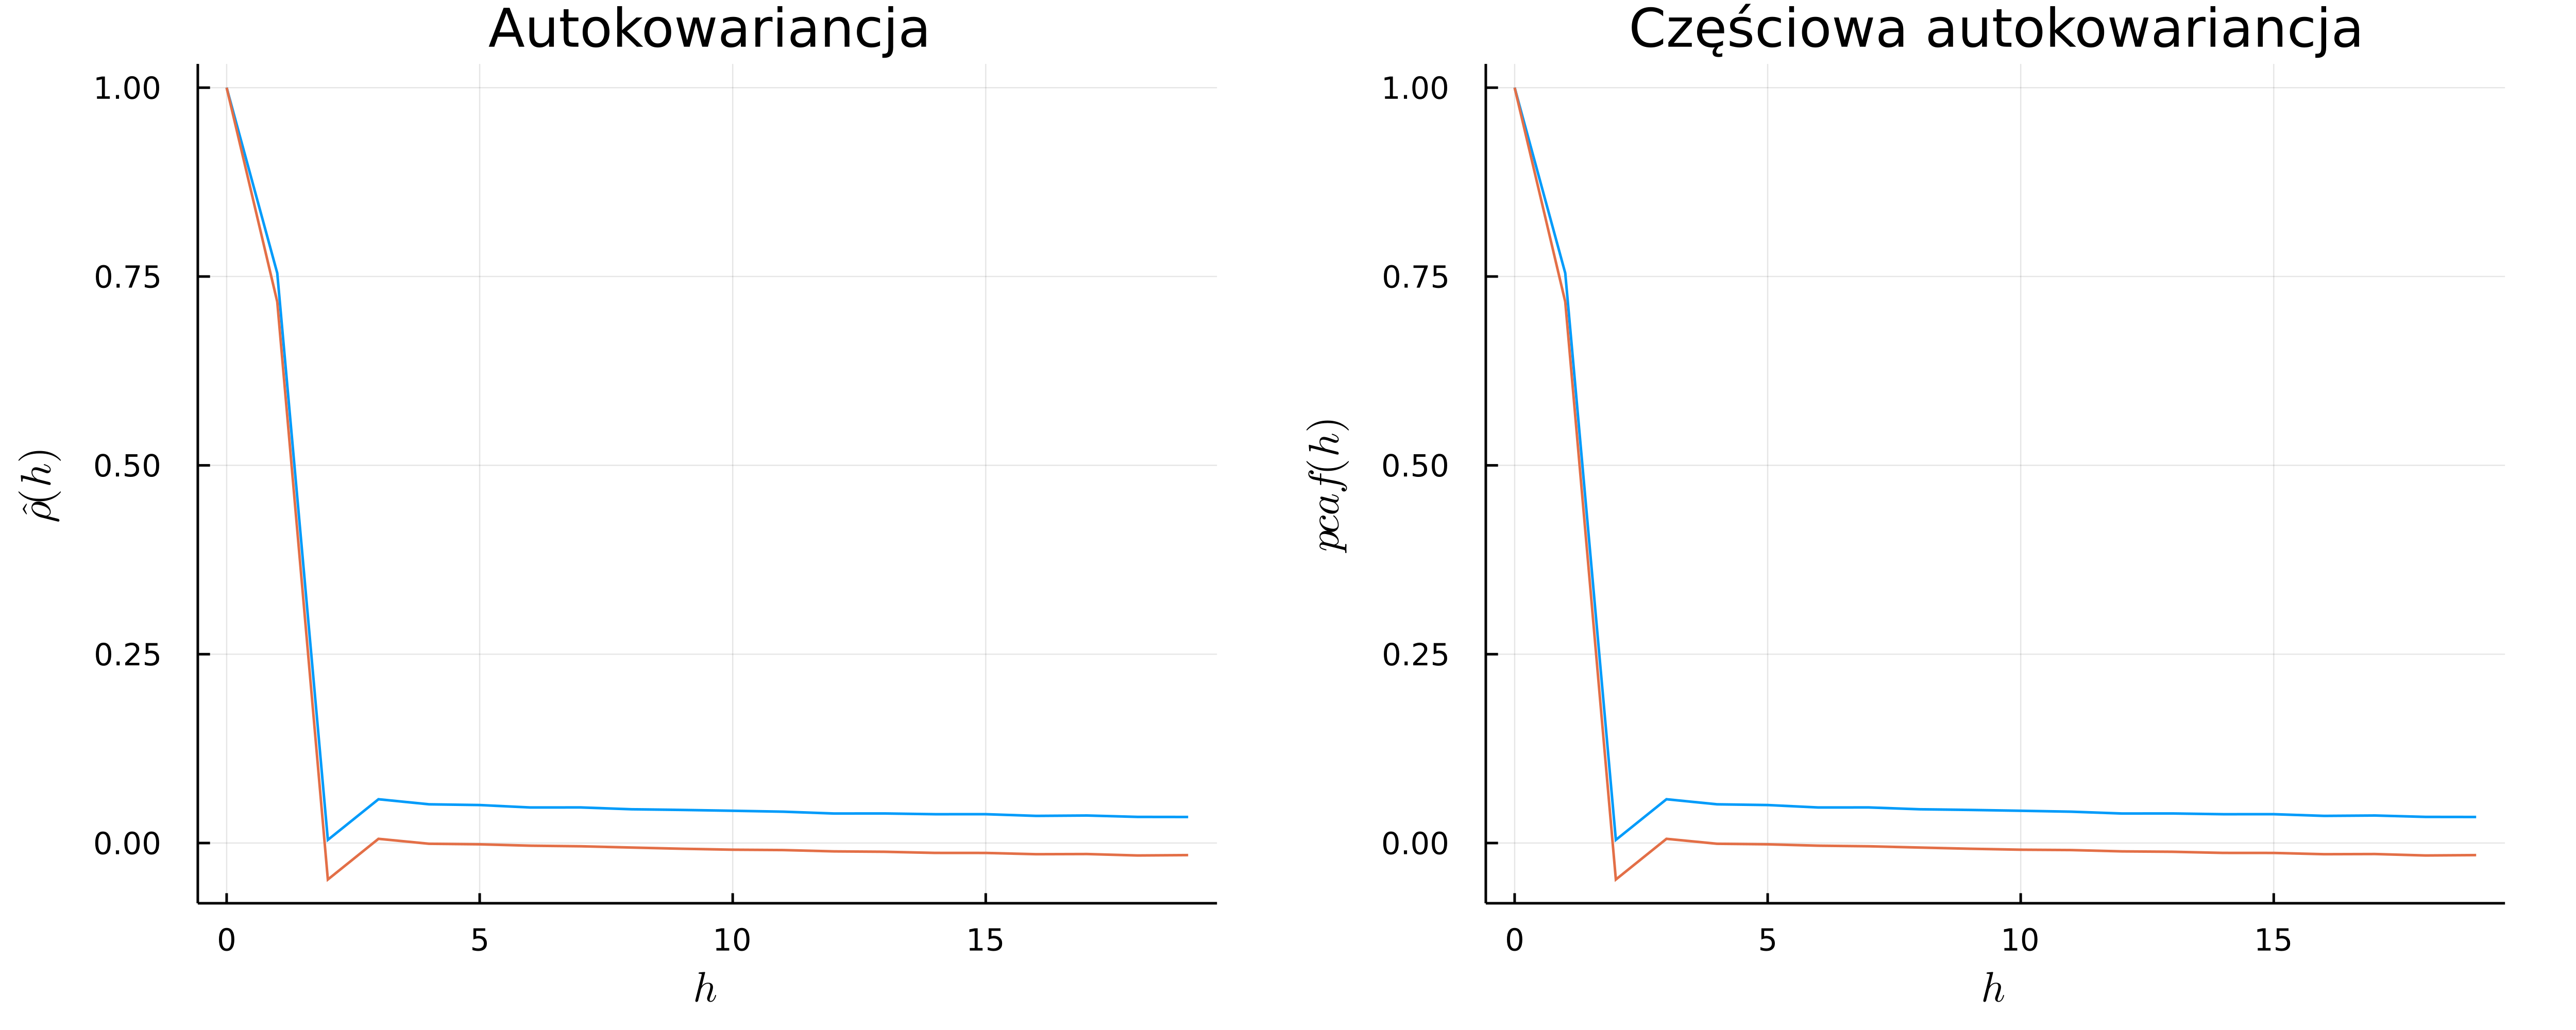
\includegraphics[width=3\columnwidth/4]{img/acf_pacf.png}
		\caption{Przedziały ufności dla ACF i PACF dla naszego modelu}
		\label{fig:model_acf_pacf}
	\end{figure}
	Jak możemy zobaczyć na wykresie \ref{fig:model_acf_pacf} istnieje tylko krótko okresowa zależność pomiędzy danymi w modelu. Ta zależność pokrywa się z naszymi oczekiwaniami, ponieważ używamy modelu ARMA(2,2) o parametrach \ref{model} gwarantujących racjonalność. 
	
	
	Następnie porównamy trajektorię z liniami kwantylowymi dla naszego modelu.
	\begin{figure}[H]
		\centering
		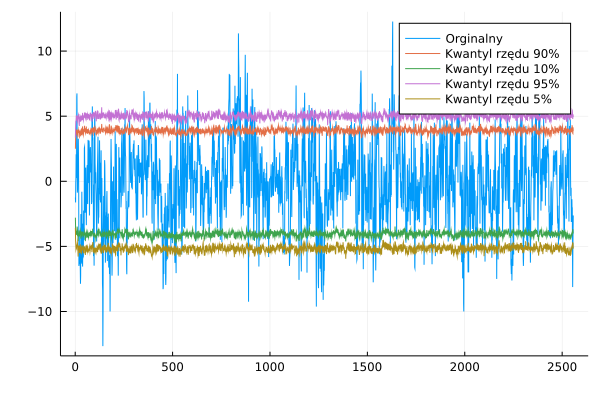
\includegraphics[width=3\columnwidth/4]{img/linie_kwantylowe.png}
		\caption{Porównanie orginalnych danych z liniami kwantylowymi modelu}
		\label{fig:linie_kwantylowe}
	\end{figure}
Analizując linie kwantylowe naszego modelu,wyznaczone również  za pomocą symulacji Monte Carlo, pokazane na wykresie \ref{fig:linie_kwantylowe} możemy zauważyć, że model w miarę dobrze się sprawdza dla naszych danych. $80\%$ danych leży pomiędzy linią kwantylową rzędu $0.9$ i $0.1$. Natomiast $89\%$  danych leży pomiędzy linią kwantylową rzędu $0.95$ i $0.05$


Patrząc na wykres zależności w modelu \ref{fig:model_acf_pacf} oraz na wykres z liniami kwantylowymi \ref{fig:linie_kwantylowe} dochodzimy do wniosku, że model dobrze się sprawdza dla naszych danych.


	\section{Analiza szumu}
	Podczas tworzenia modelu ARMA i późniejszej analizy zakładaliśmy następujące warunki odnośnie szumu
	\begin{enumerate}
		\item $\mathbb{E}\xi_i=0$ $\forall i$ ,
		\item $Var\xi_i=\sigma^2<\infty\quad\forall i$,
		\item $\xi_i\perp\!\!\!\perp\xi_j$ dla $i\neq j$,
		\item $\xi_i$ mają rozkład normalny,
	\end{enumerate}
	
	\subsection{Stała średnia równa 0}
	Sprawdzimy, czy residua naszego modelu mają stałą średnią równą $0$. W tym celu zobaczymy jak wyglądają nasze wartości resztowe.
	
	\begin{figure}[H]
	\centering
	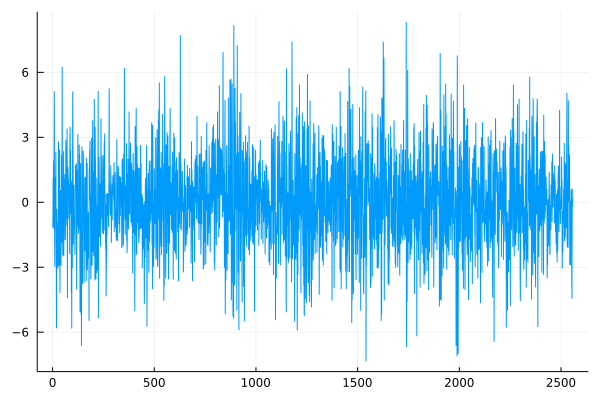
\includegraphics[width=3\columnwidth/4]{img/residua.png}
	\caption{Residua naszego modelu}
	\label{fig:residua}
\end{figure}
 Jak możemy zobaczyć na wykresie \ref{fig:residua} średnia jest stała w czasie i wynosi w przybliżeniu $0$  a dokładnie $ 7.9 \cdot 10^{-4}$. 
 W celu upewnienia się wykonamy też t test dla jednej zmiennej.
 	\begin{figure}[H]
 	\centering
 	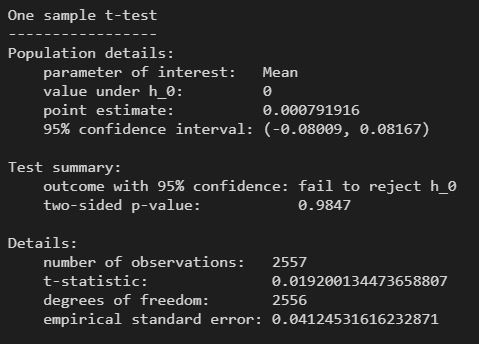
\includegraphics[width=3\columnwidth/4]{img/t_test.png}
 	\caption{Test t dla naszych wartości resztowych}
 	\label{t_test}
 \end{figure}
Jak możemy zobaczyć test t \ref{t_test} nie miał podstaw do odrzucenia hipotezy zerowej, która mówiła ,że średnia wynosi $0$. Test zwrócił $p$-value równe $0.9847$ co jest bardzo dużą wartością.
Tak więc z pewnością możemy przyjąć, że średnia jest stała i równa $0$

\subsection{Stała wariancja}
Z wykresu \ref{fig:residua} możemy odczytać,także że wariancja jest stała. Dodatkowo możemy obliczyć ,że  należy ona do przedziału $[4.141 ; 4.554]$ na poziomie ufności $\alpha = 5\%$

\subsection{Niezależność szumu}
Sprawdzimy teraz założenie dotyczące niezależności szumu w czasie. Sprawdzimy na początek wykres autokowariancji i częściowej autokowariancji. 
\begin{figure}[H]
	\centering
	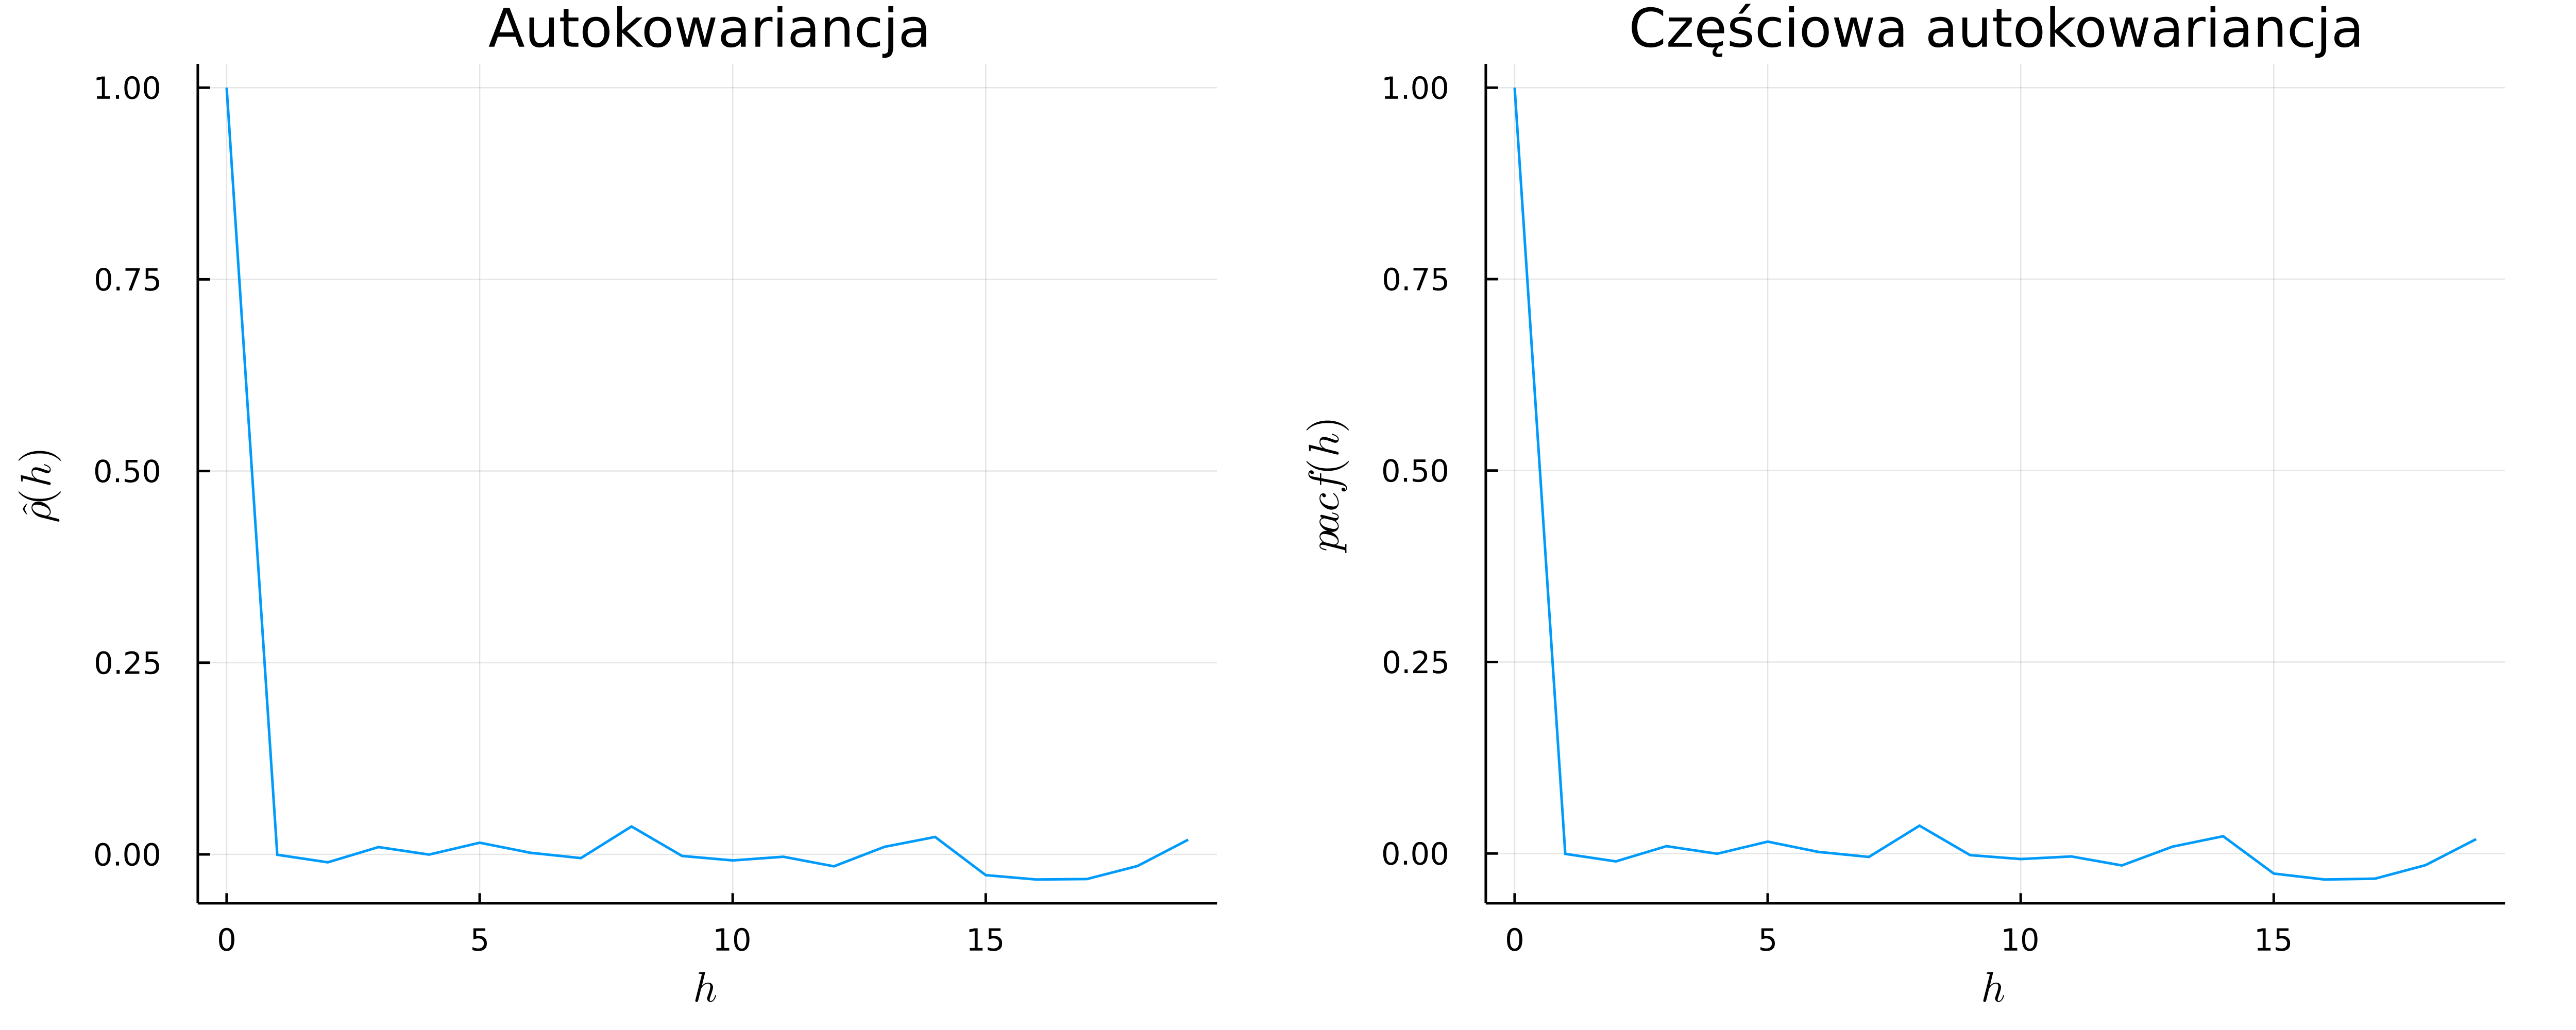
\includegraphics[width=3\columnwidth/4]{img/acf_pacf_residua.png}
	\caption{ACF i PACF dla wartości resztkowych modelu}
	\label{fig:residua_acf_pacf}
\end{figure}
Na wykresie \ref{fig:residua_acf_pacf} możemy  zobaczyć, że mamy szum jest zależny tylko od siebie w tym samym momencie, ponieważ tylko dla $h=0$ ACF oraz PACF przyjmują wartość niebędącą w otoczeniu zera.

Dodatkowo wykonamy test Ljunga-Boxa by upewnić się, że szum jest niezależny od siebie. 
\begin{figure}[H]
	\centering
	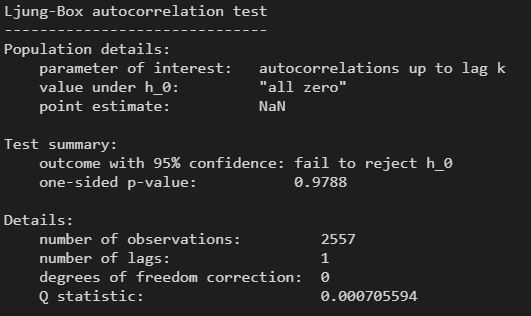
\includegraphics[width=3\columnwidth/4]{img/Ljung-Box.png}
	\caption{Test Ljunga Boxa dla naszych wartości resztowych}
	\label{Test Ljunga Boxa}
\end{figure}

Test nam potwierdza, że nie mamy podstaw do odrzucenia hipotezy mówiącej, że szum jest niezależny od siebie. Otrzymaliśmy $p$-value równe $0.9847$ co jest bardzo dużą wartością.

Łącząc wykres \ref{fig:model_acf_pacf} oraz test Ljunga Boxa stwierdzamy, że szum jest niezależny.

\subsection{Założenie o normalności rozkładu}
Sprawdzimy teraz założenie mówiące o tym, że szum ma rozkład normalny.
Na początku sprawdzimy histogram wraz z gęstością empiryczną i teoretyczną rozkładu normalnego.
\begin{figure}[H]
	\centering
	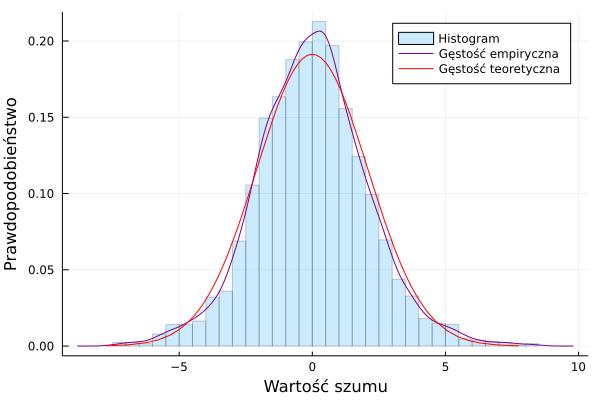
\includegraphics[width=3\columnwidth/4]{img/density.png}
	\caption{Histogram, gęstość rozkładu szumu wraz z rozkładem normalnym}
	\label{fig:density}
\end{figure}

Patrząc na histogram wraz z gęstościami \ref{fig:density} możemy załuważyć, że rozkład wartości resztowych może być normalny ale nie musi. W celu dalszego sprawdzenia normalności zobaczymy jak będzie wyglądał wykres kwantylowy.

\begin{figure}[H]
	\centering
	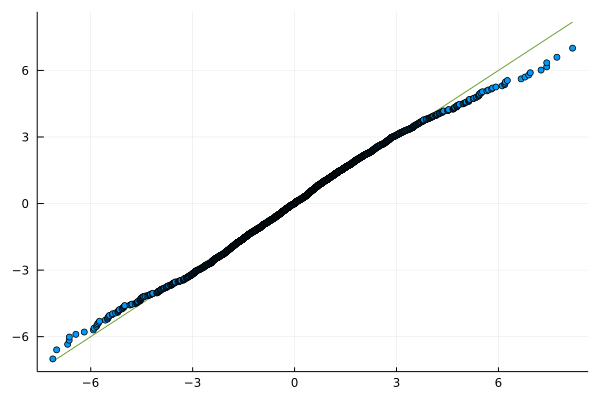
\includegraphics[width=3\columnwidth/4]{img/qqplot.png}
	\caption{Qqplot dla wartości resztowych}
	\label{fig:qqplot}
\end{figure}

Analizując wykres kwantylowy \ref{fig:qqplot} widzimy, że potencjalnie ogony rozkładu nie zgadzają się z rozkładem normalnym. W celu ostatecznej weryfikacji normalności wykonamy test Andersona Darlinga. 
\begin{figure}[H]
	\centering
	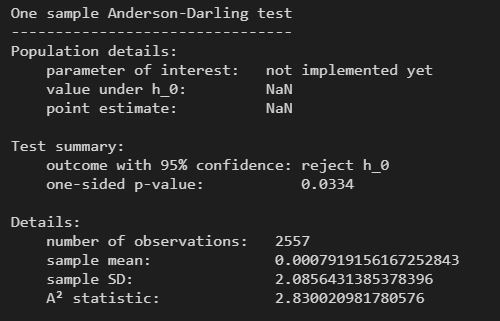
\includegraphics[width=3\columnwidth/4]{img/ad_test.png}
	\caption{Test Andersona Darlinga dla naszych wartości resztowych}
	\label{Test_AD}
\end{figure}
Test Andersona Darlinga \ref{Test_AD} odrzuca hipotezę o normalności rozkładu. Dla naszych danych $p$-value wynosi $3.3\%$. 

Podsumowując rozkład szumu nie ma rozkładu normalnego.
	\section{Wnioski autorów}
	Pogodę w Indiach po odpowiednich przekształceniach można modelować modelem ARMA. W naszym przypadku udało się za modelować modelem o wartościach $p,q = 2$ \ref{model}. Parametry modelu mówią nam, że jest on stacjonarny i przyczynowy co pokrywa się z dalszymi testami. Model spełnia założenia, lecz biały szum nie ma rozkładu normalnego. Dużym atutem modelu jest fakt, że wykorzystuje on tylko dwie średnie temperatury z dwóch ostatnich dni. Warto pamiętać, że nadal jest to proces losowy więc nigdy temperatura nie będzie dokładnie się zgadzać z modelem. 
	
\end{document}